\begin{figure}[tbp]
  \centering
  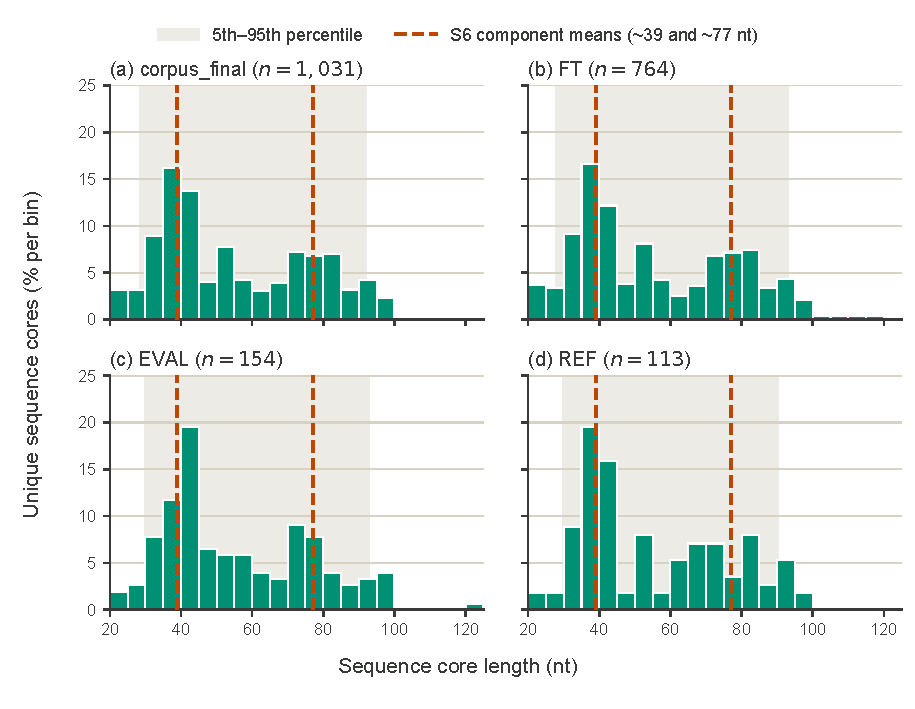
\includegraphics[width=\textwidth]{figures/final_corpus_length_distribution.pdf}
  \caption[Sequence core-length distributions for the final corpus and its partitions.]{%
  Sequence core-length distributions for (a) the complete final corpus, (b)
  FT, (c) EVAL, and (d) REF. Histograms show the relative frequency of unique
  sequence cores in 5-nt bins, so a core associated with multiple targets is
  counted once within each panel. The complete corpus contains 1,031 unique
  sequence cores, partitioned without overlap into FT ($n=764$), EVAL
  ($n=154$), and REF ($n=113$), which reconcile to the corpus total. Shaded
  regions mark the panel-specific 5th--95th percentile intervals, and dashed
  lines mark the two S6 Gaussian-mixture component means of approximately 39
  and 77 nt. Length regime was one of the four objectives used to balance the
  S7 split, so the similarity of the profiles is expected by design; the
  corresponding per-partition regime counts are reported in Table~2.}
  \label{fig:final-corpus-length-distribution}
\end{figure}
